
\subsection{ogreWatcher}

Grr! Arg!

\begin{figure}
\centering
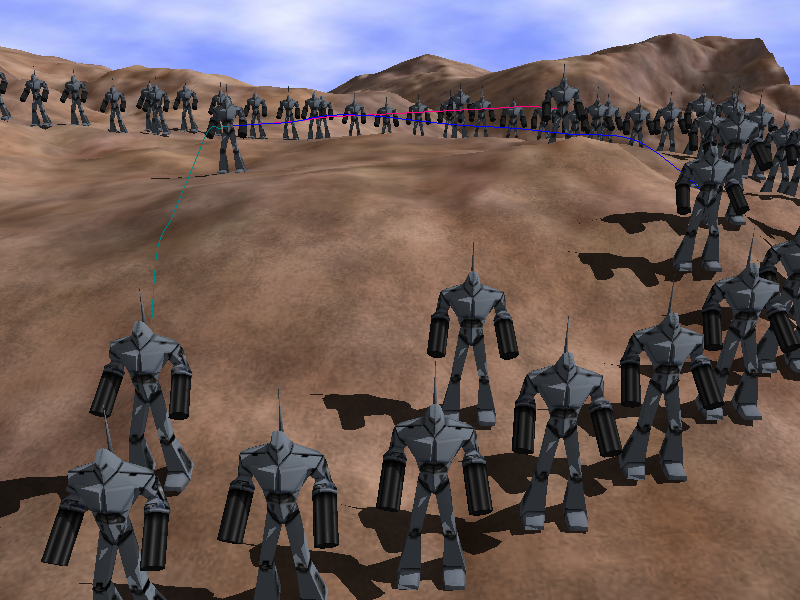
\includegraphics[width=0.8\textwidth]{ogreWatcherGUI.eps}
\caption{The ogreWatcher showing a running instance of showClock.}
\label{ogreWatcher}
\end{figure}

Built with OGRE.

\subsubsection{Configuration}

\begin{itemize}
\item {\tt -h} or {\tt --help}, show a usage message and exit. 
\item {\tt -c configfile}, gives the location of the configuration file. If not given a default one will be created, used, and saved on program exit.
\end{itemize}

\subsubsection{Command Line Options}

\begin{itemize}
\item {\tt server}, name or ipaddress of the server to connect to.
\item {\tt service}, name of service (usaully "watcherd") or port number on which the server is listening.
\end{itemize}
